%	CHAP Limma Voom
%----------------------------------------------------------------------------------------

\chapterimage{blue-chapter-head_4-reduced.pdf} % Chapter heading image

\chapter{Limma Voom}\label{chap:LimmaVoom}

\begin{remark}
Limma Voom is a statement introduced in MetaR 1.3.
\end{remark}
\section{Overview}
The Limma Voom statement makes it possible to use the Limma R package and the Limma Voom adjustment to analyze RNA-Seq data with Limma. Similarly to EdgeR, the language that provides the \texttt{Limma Voom} statement must be added to the model where you plan to use the statement in analysis. The name of the language is \textit{org.campagnelab.metar.limma}. Note that this language depends on \textit{org.campagnelab.metar.models}, which should also be imported.


\section{The Limma Voom Statement}
The \texttt{limma voom} statement performs tests of differential expression using read counts contained in a table of data. The statement has the following attributes. Figure~\ref{fig:NewLimmaVoom} presents a newly created Limma Voom statement.
\begin{figure}[h!tbp]
  \centering
  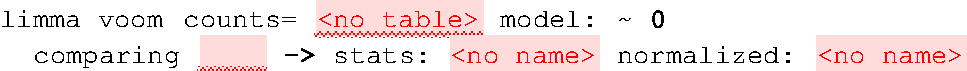
\includegraphics[width=\figWidthWide]{figures/NewLimmaVoom.pdf}
\caption[New Limma Voom Statement.]{\textbf{New Limma Voom Statement.}}
\label{fig:NewLimmaVoom}
\end{figure}
\paragraph{counts table}
The table must contain columns annotated with the ``counts'' group. Bind this table reference to a table that contains non-normalized read counts.

\paragraph{model}
You can use the model attribute to enter a linear model. Limma Voom will use this model to model the mean and variance of the data. You can enter a linear model by typing \texttt{+} followed by the name of a group usage attached to the counts table. Repeat to add multiple factors to the model. 

\paragraph{comparing}
The comparing attribute makes it possible to define the statistics that should be tested for difference with zero. After you have defined a model with several factors (corresponding to group usage), the factor levels (corresponding to group names) will be offered for auto-completion. The factor level name stands for the average of the columns annotated with the group. See Figure~\ref{fig:LimmaVoomExample} for an example. 

\paragraph{normalized}
This attribute holds a table of normalized counts that will be produced when the \texttt{limma voom} statement is executed. You should name the table of normalized counts to make it possible to reference it later. Normalized counts are available even when the model has a single factor (in which case adjust counts would not work because there is no batch to remove).

\paragraph{adjusted counts}
This attribute is exposed under the Inspector Tab(\inspectorTabIcon). It takes a boolean value: either true or false. When true, the limma voom statement will produce a table of adjusted counts. Data in this table is adjusted to remove the effect of covariates described in the model, but not used in the comparing attribute. This is useful to remove the effect of batches, or other cofactors expected to affect expression. Adjusted counts are implemented with the Limma removeBatches function.   
 
\section{Example}
Figure~\ref{fig:LimmaVoomExample} presents an example where the \texttt{Limma Voom} statement configured with a model (one factor: \texttt{LPS}) to call differences between columns labeled with the groups \texttt{LPS=YES} and \texttt{LPS=NO}.



\begin{figure}[h!tbp]
  \centering
  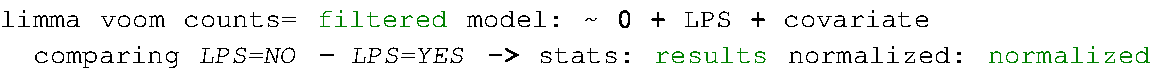
\includegraphics[width=\figWidthWide]{figures/LimmaVoomExample.pdf}
\caption[Limma Voom Example.]{\textbf{Limma Voom Example.}  Since version 1.8, limma voom outputs normalized counts.\index{New in MetaR 1.8}}
\label{fig:LimmaVoomExample}
\end{figure}

